83. $f(x)=\cfrac{1-|x-2|}{x}=\begin{cases} \cfrac{1+x-2}{x},\ x\leqslant2,\\
\cfrac{1-x+2}{x},\ x>2.\end{cases}=\begin{cases} 1-\cfrac{1}{x},\ x\leqslant2,\\
-1+\cfrac{3}{x},\ x>2.\end{cases}$\\
а) $$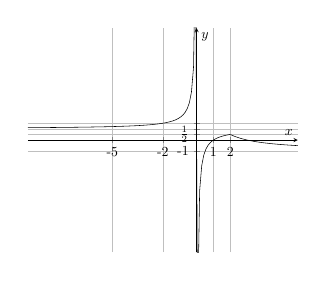
\begin{tikzpicture}[scale=0.5]
\begin{axis}[
    axis lines = middle,
    grid=major,
    legend pos={south west},
    xlabel = {$x$},
    %xlabel style={below right},
    ylabel = {$y$},
    ymin=-10,
    ymax=10,
    xmin=-10,
    xmax=6,
    xtick={-5, -2,  1, 2},
    xticklabels={-5, -2, 1, 2},
    ytick={-1, 0.5, 1, 1.5},
    yticklabels={-1, $\frac{1}{2}$, $ $, $  $},
                  ]
	\addplot[domain=-10:2, samples=100, color=black] {1-1/x};
    \addplot[domain=2.01:10, samples=100, color=black] {-1+3/x};
        %\addplot[domain=2.01:6, samples=100, color=black] {2/(2-x)};
   % \addplot[domain=-3:3, samples=100, color=black] {-x};
     %\addlegendentry{$\text{Рис. 1}$};
\end{axis}
%\draw (5.71,2.59) circle (2pt);
%\draw (3.45,0.75) circle (2pt);
%\draw (3.45,2.55) circle (2pt);
\end{tikzpicture}$$
б) При $x>0$ график функции находится ниже уровня $y=\cfrac{3}{2}.$ Если $1-\cfrac{1}{x}=\cfrac{3}{2},$ то $\cfrac{1}{x}=-\cfrac{1}{2},\ x=-2.$ Значит, $f(x)\leqslant \cfrac{3}{2}$ при $x\in(-\infty;-2]\cup(0;+\infty).$\\
в) Горизонтальными асимптотами являются $y=-1$ и $y=1,$ исходя из этого найдём количество решений: при $a\in\left(\cfrac{1}{2};1
ight]:0,$ при $a\in(-\infty;-1]\cup\left\{\cfrac{1}{2}
ight\}\cup(1;+\infty):1,$ при $a\in\left(-1;\cfrac{1}{2}
ight):2.$\\
